% !TEX TS-program = pdflatex
% !TeX encoding = UTF-8
% !TeX spellcheck = en_GB
%======================================================================
%==  template for LaTeX presentation  =================================
%======================================================================
\providecommand{\PathP}{../gotham-example/} 	% Path to Parts folders
\providecommand{\PathR}{../../resources/} 	% Path to Resources folders
\providecommand{\PathSO}{../../sources/} 	% Path to Sources folders
\providecommand{\PathS}{../../supplies/} 	% Path to Supplies folders
\providecommand{\BuildTrigger}{buildnew} 	% Trigger to build or not standalone parts.
\providecommand{\langue}{french}  % english, french

\makeatletter
	\ifx\c@levelstanda\undefined 	% to create a newcounter if it doesn't exists.
		\newcounter{levelstanda}
		\def\input@path{ {\PathSO}{\PathSO/gotham}{\PathSO/UGE/}{\PathSO/Inria/}{\PathSO/CEA/} }  % to be able to find package in source folders.
	\else
		{}% it already exist
	\fi
\makeatother


\documentclass[notheorems, noamsthm, aspectratio=43, 10pt]{beamer}
	% use this instead for 16:9 aspect ratio: [aspectratio=169]
	% supported aspect ratios  1610  169 149 54 43 (default) 32
	%
	% The option "handout, " allows to the print the hidden slides made by <handout:1|beamer:0>[noframenumbering].
	%
	% the option "notes=only, " to print only the notes !
	\usepackage[l2tabu, orthodox]{nag}	% Help to prevent buggus with warnings

%-=-=-=-=-=-=-=-=-=-=-=-=-=-=-=-=-=-=-=-=-=-=-=-=
%        DEFAULT PACKAGES
%-=-=-=-=-=-=-=-=-=-=-=-=-=-=-=-=-=-=-=-=-=-=-=-=
	\usepackage[utf8]{inputenc}
	\usepackage[T1]{fontenc}


%-=-=-=-=-=-=-=-=-=-=-=-=-=-=-=-=-=-=-=-=-=-=-=-=
%        BEAMER OPTIONS
%-=-=-=-=-=-=-=-=-=-=-=-=-=-=-=-=-=-=-=-=-=-=-=-=
	% Gotham Theme
	\usetheme{gotham}
	\usetheme{gothamUGE}
		\UgeSet{unofficial}% {official,unofficial}
	% \usetheme{gothamInria}
	% 	\InriaSet{old1}% {RF,old1,old2,old3}
	% \usetheme{gothamCEA}
	% 	\CEASet{official}% {official}

		% Apply all Gotham setting.
		\gothamset{
			% format frametitle=titlecase,
			% format title=titlecase, format section=titlecase,
			% sectionframe default=on, sectiontocframe default=on,
			numbering= totalframenumber, %none, framenumber,
			progressbar position= foot, %none, head, frametitle, foot
			background= dark, %dark, %light, %transparent,
		}


%-=-=-=-=-=-=-=-=-=-=-=-=-=-=-=-=-=-=-=-=-=-=-=-=
%        LOADING MY PACKAGES
%-=-=-=-=-=-=-=-=-=-=-=-=-=-=-=-=-=-=-=-=-=-=-=-=
		\newcommand{\Pathbasebib}{\PathR/Presentation.bib}
		\newcommand{\PathSymbolsEntries}{\PathR/UsersSymbolsAcronyms}%.bib
		\def\OSvar{linux} % windows, mac, linux
	%%%% 		UsersPackagesCommands.tex
%%%%		version 0.1.1 du 01/11/2023
%%%% 		Author: Romain NOËL
%%%%		email: romain.noel@univ-eiffel.fr
%%%%--------------------------------------------%%%%

%%%%---- OS & FONT     -------------------------%%%%
%%%%---- POLICE     ----------------------------%%%%
%%%%---- TEXT FORMATTING -----------------------%%%%
	% \usepackage{enumitem}
	% \usepackage{ulem}

	%%%% Personal %%%%
	\makeatletter
		\newcommand{\ie}{\@ifstar{\emph{i.e.\@}}{\emph{id est}\ }}
		\newcommand{\eg}{\@ifstar{\emph{e.g.\@}}{\emph{exempli gratia}\ }}
		\newcommand{\cad}{\@ifstar{c.-\`a.-d.\@}{c'est-à-dire}\ }
		\newcommand{\cf}{\@ifstar{\emph{cf.\@}}{\emph{confer}\ }}
	\makeatother

	\ExplSyntaxOn
		% Create a new command to fake Small Caps by scaling uppercase with one mandatory argument.
		\DeclareDocumentCommand{\fakesc}{ m }{
			\textapperance_smallcaps:n { #1 }
		}

		%–– user-adjustable scaling parameters
		\tl_new:N \l__fauxsc_hscale_dim  \tl_set:Nn \l__fauxsc_hscale_dim {.83}
		\tl_new:N \l__fauxsc_vscale_dim  \tl_set:Nn \l__fauxsc_vscale_dim {.72}%.72

		\tl_new:N \l__textapperance_textsmallcaps_input_tl% Initialize string variable
		\cs_new_protected:Npn \textapperance_smallcaps:n #1 {
			% Fully expand contents and store them in the variable
			\tl_set:Nx \l__textapperance_textsmallcaps_input_tl { #1 }
			
			% Replace everything thats NOT a capital letter NEITHER punctuation by \textsmaller[2]{\uppercase{<match>}}
			\regex_replace_all:nnN { ([^A-Z\ \,\.\;\:\!\?\'\"\(\)\[\]\{\}0-9]+) }{ 
				% { \c{relscale}{0.75}\cB\{\c{uppercase}\cB\{\0\cE\}\cE\}} } 
				\c{scalebox}{
					\c{l__fauxsc_hscale_dim}}[\c{l__fauxsc_vscale_dim}]{
					\cB\{\c{uppercase}\cB\{\0\cE\}\cE\}
				}
			} \l__textapperance_textsmallcaps_input_tl 
			\tl_use:N \l__textapperance_textsmallcaps_input_tl % print the result
		}

		% Adapt some language element to the command \langue.
		% Test: does \langue exist?
		\cs_if_exist:cTF { langue }{
			% Yes, it exists.  
			% Now compare its expansion to the string "french".
			\str_if_eq:VnTF \langue { french }{
				% ⟨true⟩ branch so its adapt some commands
				\renewcommand{\partContentName}{Contenu\ de\ la\ partie}
				\renewcommand{\secContentName}{Contenu\ de\ la\ section}
				\renewcommand{\subsecContentName}{Contenu\ de\ la\ sous-section}
			}{
				% ⟨false⟩ branch (exists but isn’t “french”) so do nothing
			}
		}{
			% Command doesn’t exist
			\typeout{\string\langue~does~not~exist.}
		}
	\ExplSyntaxOff

	\newcommand{\famName}[1]{\fakesc{#1}}%\textsc


%%%%---- SPACING & JUSTIFICATION ---------------%%%%
%%%%---- LAYOUT & MARGINS ----------------------%%%%
	\usepackage{changepage}
   \usepackage{appendixnumberbeamer} % Manage frame numbering in appendixes in beamer


%%%%---- FOOT PAGE & HEAD ----------------------%%%%
%%%%---- TABLE of CONTENT & FIGURES ------------%%%%
%%%%---- PARTS & CHAPTERS ----------------------%%%%
%%%%---- WATERMARKS ----------------------------%%%%
%%%%---- COVER PAGE ----------------------------%%%%
%%%%---- IMAGES --------------------------------%%%%
	%\usepackage{placeins} % provide FloatBarrier
	%\usepackage[absolute,overlay]{textpos} % for positioning text or floats at absolute coords.
	\usepackage{float} % finer control of float and new float env
	\usepackage{subcaption} % multiple figures
		%\renewcommand{\thesubfigure}{{\normalfont\alph{subfigure}}}%


%%%%---- DRAWING & GRAPHS ----------------------%%%%
	\usepackage{import}
	\usepackage{tikz} %
	\usepackage{pgfplots} %
		\pgfplotsset{compat=newest} %
		\pdfsuppresswarningpagegroup=1


%%%%---- TABLES & BOXES ------------------------%%%%
	% \usepackage{tcolorbox} % colored box with a lot of flexibility
	% 	\tcbuselibrary{skins,theorems} % extra for pseudo(code)
	\usepackage{tabularray} % Typeset tabulars and arrays (contains equivalent of longtable, booktabs and dcolumn at least)
		\UseTblrLibrary{booktabs} % to load extra commands from booktabs
		% \UseTblrLibrary{diagbox} % for cells with a diagbox
		% \UseTblrLibrary{varwidth} % for cell with variable width
		% \UseTblrLibrary{amsmath} % to improve with +array, +matrix, +bmatrix, +Bmatrix, +pmatrix, +vmatrix, +Vmatrix and +cases
		% \UseTblrLibrary{siunitx} % for cell using SI formatting


%%%%---- SYMBOLS -------------------------------%%%%
%%%%---- MATHS & PHYSICS -----------------------%%%%
	\usepackage{amsmath, amsfonts, amssymb} % American Math Standard
	\usepackage{mathtools} % extension of AMS with tools
	\usepackage{mleftright} % better left and right bracket management
	\usepackage{derivative} % standard and customable derivative operators
	\usepackage{siunitx} % International System units
	% \usepackage{tensorsop} % work in progress ^^
	\usepackage{amsthm, thmtools} % replacement of ntheorem
		\declaretheorem{theorem}
		% Define a theorem style that uses Beamer's 'block' environment
		\renewenvironment{theorem}[1][]{%
			\refstepcounter{theorem}% Increment the theorem counter
			\begin{block}{\thmname{Theorem}~\thmnumber{\thetheorem}\if\relax\detokenize{#1}\relax\else~(#1)\fi:}%
		}{%
			\end{block}%
		}
	% \usepackage{empheq} % emphasize equations
	\usepackage[only,llbracket,rrbracket]{stmaryrd}
	% \usepackage{bm}


%%%%---- THEOREMS ------------------------------%%%%
%%%%---- CHEMISTRY & BIO -----------------------%%%%
%%%%---- CODING, LINKS & OTHERS ----------------%%%%
	% \usepackage{listings} % to include piece of codes
	\usepackage{pseudo} % for flexible pseudocode
		\floatstyle{ruled} % create a env for algorithms with Float
		\newfloat{algorithm}{htbp}{alg}
		\floatname{algorithm}{Algorithm}
	\usepackage{cleveref}%
	\usepackage{standalone} 	% Other include compilable alone.


%%%%---- INDEX & GLOSSARIES --------------------%%%%
	\usepackage[record, automake, section=section]{glossaries-extra}
		%Newglossaries
		\newglossary*{acronym}{Abbreviations}
		\newglossary*{notation}{Notation}
		\newglossary*{symbol}{Nomenclature}

		% new keys must be defined before \GlsXtrLoadResources
		\glsaddstoragekey{unit}{}{\glsentryunit}

		% define style of the abbreviation in the text
		\setabbreviationstyle[acronym]{long-short}
		\setabbreviationstyle[foreignabbreviation]{long-short-user}
		\setabbreviationstyle[inline]{long-short}	%
		\setabbreviationstyle[footer]{footnote} 	%


		% \newcommand{\AtEndPreambPerso}{
		\GlsXtrLoadResources[
			src={\PathSymbolsEntries}, % entries in symbols.bib
			%selection=all,
			%save-locations=false,% location list not needed
			entry-type-aliases={main=entry, notation=entry, foreignabbreviation=abbreviation},
			field-aliases={
				foreignlong=user1,
				nativelong=long
			},
			type=acronym,
			match={entrytype=(acronym|abbreviation)},
			category={same as original entry}% requires bib2gls v1.4+
			%sort
		]

		\GlsXtrLoadResources[
			src={\PathSymbolsEntries}, % entries in symbols.bib
			%selection=all,
			%save-locations=false,% location list not needed
			entry-type-aliases={main=entry, notation=entry, foreignabbreviation=abbreviation},
			type=symbol,
			match={entrytype=symbol},
			sort-field={category},% sort @symbol entries by category field
			symbol-sort-fallback=description,% sort @symbol entries by name field
			identical-sort-action=name,% sort by description if sort value identical
			sort={letter-nocase},
			% symbol-sort-fallback=name,% sort @symbol entries by name field
			% identical-sort-action=description,% sort by description if sort value identical
		]
		% }
		\glsdisablehyper


%%%%---- BIBLIOGRAPHY --------------------------%%%%
	\usepackage[%citestyle=numeric,  	% style de citation : alphabetic, numeric, 		authoryear,
		%bibstyle=numeric, 	% style de la biblio : alphabetic, authoryear, numeric,
		style=numeric,			% style gloabel + apa, ieee, ams : style predefinit par certains organisme
		sorting=none,
		mcite=true,				% collapsing  multiple  citations into one
		subentry,				% have entry that referes to another (not with authoryear)
		labelnumber, 			%
		citetracker=true,		% To track citations
		% backref=true,			% afficher les pages ou les citations sont dans la biblio
		url=false,
		giveninits=true,   	% Initials for first name
		maxcitenames=3,			% nb max de noms lors de \cite, audela "et al."
		maxbibnames=100,		% nb max de noms dans la biblio, audela "et al."
		defernumbers=true,		% ne pas charger toute la base de donnees, uniquement le necessaire
		backend=biber			% bibtex, biber
	]{biblatex}

		% \AtEveryBibitem{\clearfield{url}}
		\renewcommand{\mkbibnamefamily}[1]{\textsc{#1}}

		% Let us now load the bib files.
		%% \addbibresource[datatype=bibtex]{\Pathbasebib}
		% requires etoolbox to loop from a CSV list. (etoolbox is loaded implicitly by ...)
		%\addbibresource[datatype=bibtex]{\Pathbasebib}
		\newcommand{\mylistDo}[1]{ \addbibresource[datatype=bibtex]{#1} }%
		%\forcsvlist{\mylistDo}{\expandafter\Pathbasebib}
		\expandafter\forcsvlist\expandafter\mylistDo\expandafter{\Pathbasebib}

		% Create a \defbibentrysetlabel command in order to redefine the printing of mcite manually
		\makeatletter
			% warning the file called \blxmset@bibfile@name will be
			% overwritten without warning
			\def\blxmset@bibfile@name{\jobname -msets.bib}
			\newwrite\blxmset@bibfile
			\immediate\openout\blxmset@bibfile=\blxmset@bibfile@name
			\immediate\write\blxmset@bibfile{%
				@comment{auxiliary file for \string\defbibentrysetlabel}^^J%
				@comment{This file may safely be deleted.
					It will be recreated as required.}}

			\AtEndDocument{%
				\closeout\blxmset@bibfile}

			\newrobustcmd*{\defbibentrysetlabel}[3]{%
				\@bsphack
				\immediate\write\blxmset@bibfile{%
					@set{#1, entryset = {\unexpanded{#3}}, %
						shorthand = {\unexpanded{#2}},}%
				}%
				\nocite{#1}%
				\@esphack}

			\addbibresource{\blxmset@bibfile@name}
		\makeatother

		\renewcommand{\entrysetpunct}{.\newline}

		% Change the footnote style with letters to avoid confusion.
		\renewcommand{\thefootnote}{\alph{footnote}}
		% Change the style of the printing biblio to let appear the numbers like in the footnote
		\setbeamertemplate{bibliography item}{\insertbiblabel}

		% Define the new cite command using the footnote
		\DeclareCiteCommand{\footfullciteBeamer}
		{\usebibmacro{prenote}}
		{%
			\renewcommand{\thefootnote}{\arabic{footnote}}% Switch to footnote with numbers
			\footnotemark[\thefield{labelnumber}]% Add the mark corresponding to the number entry%
			\footnotetext[\thefield{labelnumber}]{%  Add the footnote text with same number entry.
				% \printfield{labelnumber}
				\printnames{labelname}% The name
				\setunit{\printdelim{nametitledelim}}% separator
				\printfield[citetitle]{labeltitle}% The title
				\setunit{\addperiod\space}% separator
				\printfield{year}% The year
			}%
			\renewcommand{\thefootnote}{\alph{footnote}}% Switch back to footnote with letters.
		}
		{\multicitedelim}
		{\usebibmacro{postnote}}

		%
		\DeclareCiteCommand{\fullciteBeamer}
		{\usebibmacro{prenote}}
		{\printnames{labelname}%
			\setunit{\printdelim{nametitledelim}}%
			\printfield[citetitle]{labeltitle}%
			\setunit{\addperiod\space}%
			\printfield{year}%
		}
		{\multicitedelim}
		{\usebibmacro{postnote}}


%%%%---- MULTIMEDIA ---------------------------%%%%
	% from float package
		\floatstyle{plain} % create a env for algorithms with Float
		\newfloat{video}{H}{vid}
		\floatname{video}{Video}
	\usepackage{animate} % Create embedded animation from images on all OS and viewer !

		% Os variables for the macros
		%\def\OSvar{linux} % windows, mac, linux
		\def\OSlinux{linux}
		\def\OSwindows{windows}
		\def\OSmac{mac}
		\providecommand{\includeVideo}[3][]{The command includeVideo is not correctly defined for your OS.}

	%%%%%%%%%%%%%%%%%%%%%%%%%%%%%%%%%%%%%%%%
	% To convert Video with right codec !!!!
	%%%%%%%%%%%%%%%%%%%%%%%%%%%%%%%%%%%%%%%%
	% ffmpeg -i Bubble_light.avi -vf scale="trunc(iw/2)*2:trunc(ih/2)*2" -c:v libx264 -profile:v high -pix_fmt yuv420p -g 30 -r 30 Bubble_light.mp4

		% Load the useful package for linux
		\ifx\OSvar\OSlinux
			\usepackage{multimedia}

			\renewcommand{\includeVideo}[3][]{%
				\movie[ % On linux with okular ++ poppler and phonon-backend-vlc installed
					showcontrols=true, %
					%poster, %
					#1% some options like size
				]%
				{#3}%
				{#2}
			}
		\fi
		% for windows
		\ifx\OSvar\OSwindows
			\usepackage{embedvideo}
			% \usepackage{media9}

			% \renewcommand{\includeVideo}[3][]{%
			% 	\includemedia[% % Windows AcrobatReader >9.1
			% 		%	activate=pagevisible,%
			% 		%   activate=onclick, %this is default
			% 		%	deactivate=pageclose,%
			% 		addresource=#2,%
			% 		flashvars={%
			% 			src=#2 % same path as in addresource!
			% 			%	&autoPlay=true % default: false; if =true, automatically starts playback after activation (see option ‘activation)’
			% 			%	&loop=true % if loop=true, media is played in a loop
			% 			%	&controlBarAutoHideTimeout=0 %  time span before auto-hide
			% 		},%
			% 		#1% some options like size%
			% 	]{#3}{StrobeMediaPlayback.swf}% %{SlideShow.swf} %{APlayer.swf} %{StrobeMediaPlayback.swf} %{VPlayer.swf}
			% }% end of the new command
		\fi


%%%%---- TRANSLATION ---------------------------%%%%
%%%%---- VARIABLES -----------------------------%%%%
%%%%---- MACROS --------------------------------%%%%
%%%%---- HYPHENATIONS & ACRONYMS --------------%%%%

	%%%% 		UsersPackagesCommands.tex			%%%%
%%%%		version 0.0.1 du 12/12/2020			%%%%
%%%% 		Author: Romain NOËL					%%%%
%%%%		email: romain.noel@univ-eiffel.fr			%%%%
%%%%--------------------------------------------%%%%

%%%%---- OS & FONT     -------------------------%%%%
%%%%---- POLICE     ----------------------------%%%%
%%%%---- TEXT FORMATTING -----------------------%%%%
%%%%---- SPACING & JUSTIFICATION ---------------%%%%
%%%%---- LAYOUT & MARGINS ----------------------%%%%
%%%%---- FOOT PAGE & HEAD ----------------------%%%%
%%%%---- TABLE of CONTENT & FIGURES ------------%%%%
%%%%---- PARTS & CHAPTERS ----------------------%%%%
%%%%---- WATERMARKS ----------------------------%%%%
%%%%---- COVER PAGE ----------------------------%%%%
%%%%---- IMAGES & FLOAT ------------------------%%%%
%%%%---- DRAWING & GRAPHS ----------------------%%%%
%%%%---- TABLES & BOXES ------------------------%%%%
%%%%---- SYMBOLS -------------------------------%%%%
%%%%---- MATHS & PHYSICS -----------------------%%%%
		\newcommand{\Rea}{\ensuremath{\mathbb{R} }} 
		\newcommand{\Com}{\ensuremath{\mathbb{C} }} 
		\newcommand{\diff}{\ensuremath{\operatorname{d}\!}} 	% 
		\newcommand{\diffe}{\ensuremath{\operatorname{d}\!}}
		\newcommand{\diverg}{\mathop{\textrm{div}}\nolimits} 		% 
		\newcommand{\gradi}{\mathop{\textrm{grad}}\nolimits} 	%
		\newcommand{\rota}{\mathop{\textrm{rot}}\nolimits} 		%
		\DeclareMathOperator{\Tr}{Tr}
		\DeclareMathOperator{\erf}{erf}
		\DeclareMathOperator{\Diag}{diag}
		\newcommand{\adher}[1]{\overline{#1}}
		\newcommand{\norm}[2][]{\ensuremath{\Vert{#2}\Vert_{#1}}}
		\newcommand{\absval}[2][]{\ensuremath{\vert{#2}\vert_{#1}}}
		\newcommand{\prodSca}[2]{\ensuremath{\left\langle{#1}\middle|{#2}\right\rangle }}
		\newcommand{\scalar}{\ensuremath{\cdot}}
		\newcommand{\dyadic}[3][]{\ensuremath{ {#2}\otimes^{#1}{#3} }}
		\newcommand{\contra}[3][]{\ensuremath{ {#2}{\,\overset{#1}{\cvdots}}\,{#3} }}
		\newcommand{\doublecontra}[2]{\ensuremath{ {#1}\, :\,{#2} }}
		\newcommand{\transpo}[1]{\ensuremath{ {#1}^{T} }}
		\newcommand{\bigOh}[1]{\ensuremath{ \mathcal{O}\!\left({#1}\right) }}
		\newcommand{\smalloh}[1]{\ensuremath{ \omicron\!\left({#1}\right) }}
		\newcommand{\convo}[2]{\ensuremath{ {#1}\star{#2} }}
		
		\makeatletter
			\newcommand{\@parenth}[1]{\left(#1\right)}
			\newcommand{\@indexparenth}[2][]{_{#1}\left(#2\right)}
			\newcommand{\@indexparenthStar}[2][]{_{#1}\, #2}
			\newcommand{\@subsupscriparenth}[3][]{_{#1}^{#2}\left(#3\right)}
			\newcommand{\@subsupscriparenthStar}[3][]{_{#1}^{#2}\, #3}
			\newcommand{\divergN}{\nabla\@ifstar{\@divergNStar}{\@divergNNostar}}
				\newcommand{\@divergNNostar}[2][]{_{#1}\cdot\left(#2\right)}
				\newcommand{\@divergNStar}[2][]{_{#1}\cdot #2}
			\newcommand{\gradN}{\nabla\@ifstar{\@indexparenthStar}{\@indexparenth}}
			\newcommand{\LaplaN}{\mathop{}\!\nabla^2\@ifstar{\@indexparenthStar}{\@indexparenth}}
			\newcommand{\DalembN}{\mathop{}\!\mathbin\Box\@ifstar{\@indexparenthStar}{\@indexparenth}}
			\newcommand{\rotN}{\nabla\@ifstar{\@rotNStar}{\@rotNNostar}}
				\newcommand{\@rotNNostar}[2][]{_{#1}\wedge\left(#2\right)}
				\newcommand{\@rotNStar}[2][]{_{#1}\wedge #2}
			\newcommand{\divergO}{\diverg\@ifstar{\@indexparenthStar}{\@indexparenth}}
			\newcommand{\gradO}{\gradi\@ifstar{\@indexparenthStar}{\@indexparenth}}
			\newcommand{\rotO}{\rota\@ifstar{\@indexparenthStar}{\@indexparenth}}
			\newcommand{\LaplaO}{\mathop{}\!\mathbin\bigtriangleup\@ifstar{\@indexparenthStar}{\@indexparenth}}
			\newcommand{\DalembO}{\mathop{}\!\mathbin\Box\@ifstar{\@indexparenthStar}{\@indexparenth}}
			\newcommand{\gradNp}{\nabla\@ifstar{\@subsupscriparenthStar}{\@subsupscriparenth}}
		\makeatother
		
%%%%---- THEOREMS ------------------------------%%%%
%%%%---- CHEMISTRY & BIO -----------------------%%%%
%%%%---- CODING --------------------------------%%%%
%%%%---- INCLUDE OTHER FILES -------------------%%%%
%%%%---- LaTeX PROGRAMMING  --------------------%%%%
%%%%---- TESTING & EXTRA -----------------------%%%%
%%%%---- LINKS & REFERENCES --------------------%%%%
%%%%---- INDEX & GLOSSARIES --------------------%%%%
%%%%---- BIBLIOGRAPHY --------------------------%%%%
%%%%---- TRANSLATION ---------------------------%%%%
%%%%---- VARIABLES -----------------------------%%%%
%%%%---- MACROS --------------------------------%%%%

%%%%---- HYPHENATIONS & ACRONYMS --------------%%%%
  \hyphenation{an-ti-cons-ti-tu-tion-el-le-ment bal-lon di-men-sion-ne-ment}
  \hyphenation{é-qua-tion}


	% To see notes !
	%\setbeameroption{show notes} % un-comment to see the notes in
	%\usepackage{pgfpages}
	% See notes
	%\setbeameroption{show notes on second screen=right} % Requires \usepackage{pgfpages} and pympress or pdfpc


%-=-=-=-=-=-=-=-=-=-=-=-=-=-=-=-=-=-=-=-=-=-=-=-=
%	PRESENTATION INFORMATION
%-=-=-=-=-=-=-=-=-=-=-=-=-=-=-=-=-=-=-=-=-=-=-=-=
	\title[]{Univ-Eiffel Template}
	\subtitle{A modern beamer theme based on Gotham}
	\date[]{\today}
	\author[romain.noel@univ-eiffel.fr]{
		Romain NOËL\inst{1}\inst{2}
		\and John DOE\inst{3}
	}
	\institute[Univ. Eiffel]{
		\inst{1} Université Gustave Eiffel
		\and \inst{2} Inria
		\and \inst{3} An Awesome Company
	}
	\titlegraphic{
		\hspace*{0.52\textwidth}\vspace{1.6mm}%
		
\includegraphics[height=0.08\paperheight]{\PathSO/Inria/logos/inr_logo_rouge.pdf}%
	}

	\logo{
\includegraphics[width=1.5cm]{\PathSO/Inria/logos/inr_logo_rouge.pdf}}
	\addtobeamertemplate{logo}{\vspace{0.76\paperheight}}{} % Top Right
	%\addtobeamertemplate{logo}{}{\hspace{0.885\paperwidth}} % Bottom Left
	%\addtobeamertemplate{logo}{\vspace{0.72\paperheight}}{\hspace{0.885\paperwidth}} % Top Left


	\usepackage{ccicons}
	\newcommand{\themename}{\textbf{\textsc{Gotham}}}


\begin{document}
\stepcounter{levelstanda}

%%%%%%%%%%%%%%%%%%%%%
%%%  FRONTMATTER  %%%
%%%%%%%%%%%%%%%%%%%%%
	% FRAME
	%\maketitle
	\begin{frame}[plain,noframenumbering]
		\titlepage
		\note{Everything you want}
	\end{frame}

	% FRAME
	\begin{frame}[toc]{Outline}
		\begin{columns}[T,onlytextwidth]
		\column{0.65\textwidth}
			\tableofcontents[hideallsubsections]
		\column{0.275\textwidth}
			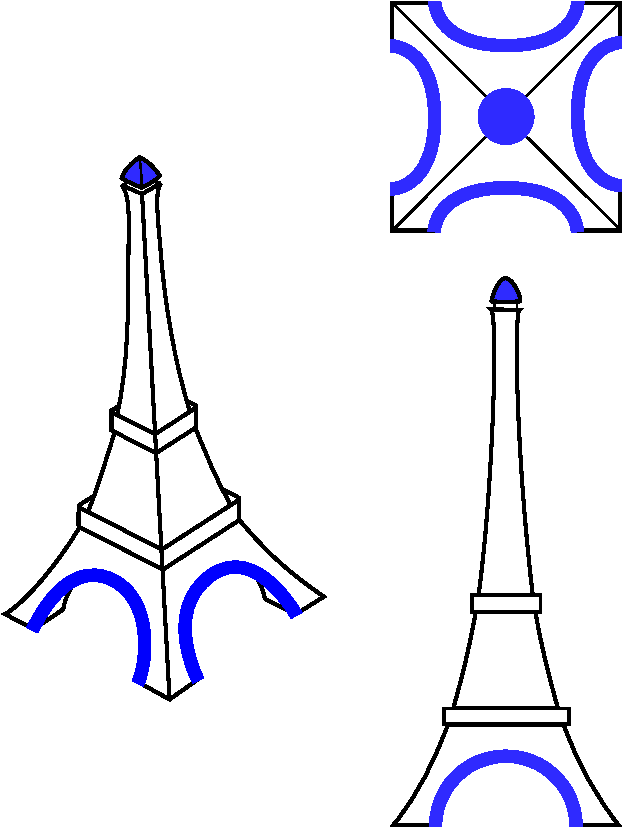
\includegraphics[width=0.99\textwidth]{\PathSO/UGE/logos/EiffelTower.pdf}
		\end{columns}
	\end{frame}


%%%%%%%%%%%%%%%%%%%%
%%%  MAINMATTER  %%%
%%%%%%%%%%%%%%%%%%%%
\documentclass[aspectratio=169]{beamer}

	\usepackage{standalone}
	\usepackage{tikz}
	\usepackage{pgfplots}

	\usepackage{tabularray} % Typeset tabulars and arrays (contains equivalent of longtable, booktabs and dcolumn at least) 
		\UseTblrLibrary{booktabs} % to load extra commands from booktabs

	\usepackage{natbib}
\begin{filecontents*}[overwrite]{pres.bib}
@article{Knuth92,
	author = "D.E. Knuth",
	title = "Two notes on notation",
	journal = "Amer. Math. Monthly",
	volume = "99",
	year = "1992",
	pages = "403--422",
}

@book{ConcreteMath,
	author = "R.L. Graham and D.E. Knuth and O. Patashnik",
	title = "Concrete mathematics",
	publisher = "Addison-Wesley",
	address = "Reading, MA",
	year = "1989"
}

@unpublished{Simpson,
	author = "H. Simpson",
	title = "Proof of the {R}iemann {H}ypothesis",
	note = "preprint (2003), available at \texttt{http://www.math.drofnats.edu/riemann.ps}",
	year = "2003"
}

@incollection{Er01,
	author = "P. Erd{\H o}s",
	title = "A selection of problems and results in combinatorics",
	booktitle = "Recent trends in combinatorics (Matrahaza, 1995)",
	publisher = "Cambridge Univ. Press",
	address = "Cambridge",
	pages = "1--6",
	year = "1995"
}

@article{greenwade93,
	author  = "George D. Greenwade",
	title   = "The {C}omprehensive {T}ex {A}rchive {N}etwork ({CTAN})",
	year    = "1993",
	journal = "TUGBoat",
	volume  = "14",
	number  = "3",
	pages   = "342--351"
}
\end{filecontents*}


\begin{document}

\section{Introduction: Beamer}

	% FRAME
	\begin{frame}[fragile]{Title page}
		The Title page is printed using the command:			
		\begin{verbatim}    \maketitle\end{verbatim}
		
		The element printed on this page are defined in the preamble by
		\begin{verbatim}
			\title[]{Gotham}
			\subtitle{A Modern, versatile and extendable theme for Beamer}
			\date[]{\today}
			\author[]{Romain NOËL}
			\institute{Center for modern beamer themes}
			\titlegraphic{\hfill\includegraphics[height=1.5cm, draft]{Title_logo.pdf}}
		\end{verbatim}
	\end{frame}
	
	% FRAME
	\begin{frame}[fragile]{Plain Slide}
		The usual page is printed and defined using the command:			
		\begin{verbatim}
			\begin{frame}{Title on top of the frame}
				contenu...
			\end{frame }
		\end{verbatim}
		
		Note that the logo printed on this page are defined in the preamble by
		\begin{verbatim}
			\logo{
\includegraphics[height=1.5cm, draft]{logo.pdf}}
		\end{verbatim}
	\end{frame}

	% FRAME
	\begin{frame}[fragile]{Sections}
		Sections group slides of the same topic
		
		\begin{verbatim}    \section{Elements}\end{verbatim}
	\end{frame}

	% FRAME
	\begin{frame}[fragile]{Typography}
		\begin{verbatim}
			The theme provides sensible defaults to
			\emph{emphasize} text, \alert{accent} parts
			or show \textbf{bold} results.
		\end{verbatim}
		
		\begin{center}becomes\end{center}
		
		The theme provides sensible defaults to \emph{emphasize} text,
		\alert{accent} parts or show \textbf{bold} results.
	\end{frame}
		
	% FRAME
	\begin{frame}{Font feature test}
		\begin{itemize}
			\item Regular
			\item \textit{Italic}
			\item \textsc{Small Caps}
			\item \textbf{Bold}
			\item \textbf{\textit{Bold Italic}}
			\item \textbf{\textsc{Bold Small Caps}}
			\item \texttt{Monospace}
			\item \texttt{\textit{Monospace Italic}}
			\item \texttt{\textbf{Monospace Bold}}
			\item \texttt{\textbf{\textit{Monospace Bold Italic}}}
		\end{itemize}
	\end{frame}
		
	% FRAME
	\begin{frame}{Lists}
		\begin{columns}[T,onlytextwidth]
			\column{0.33\textwidth}
				Items
				\begin{itemize}
		  			\item Milk \item Eggs \item Potatoes
					\begin{itemize}
						\item Milk \item Eggs \item Potatoes
						\begin{itemize}
							\item Milk
						 \end{itemize}
				 	\end{itemize}
				\end{itemize}
			
			\column{0.33\textwidth}
				Enumerations
				\begin{enumerate}
		  			\item First, \item Second and \item Last.
				\end{enumerate}
			
			\column{0.33\textwidth}
				Descriptions
				\begin{description}
		  			\item[PowerPoint] Meeh. \item[Beamer] Yeeeha.
				\end{description}
		\end{columns}
		
		\vspace{2em}
		Then, something below the columns, that be long enough to recover all the line-width.
	\end{frame}
	
	% FRAME
	\begin{frame}{Animation}
		\begin{itemize}[<+- | alert@+>]
			\item \alert<4>{This is\only<4>{ really} important}
			\item Now this
			\item And now this
		\end{itemize}
	\end{frame}

	% FRAME from https://www.edpif.org/documents/latex/intermediate/beamer/latex-int-beamer_handout.pdf
	\begin{frame}[fragile]{Commands controlling overlay}
		Beamer defines a bunch of commands intended to control overlays:
		\verb$\only<...>{text}$ Throws away \verb$text$ content on slides not in \verb$<...>$
		\verb$\onslide<...>{text}$ Same, but when hidden \verb$text$ still takes space.
		\verb$\visible<...>{text}$ Same.
		\verb$\uncover<...>{text}$ Same, but also handle transparency.
		\verb$\invisible<...>{text}$ Opposite of \verb$\visible$
		\verb$\alt<...>{text1}{text2}$ Alternates between \verb$text1$ and \verb$text2$ for\verb$ <...>$.
		\verb$\temporal<...>{before}{inside}{after}$ Alternate between three texts	depending on slide index before, inside or after the range of \verb$<...>$.
		For the commands \verb$\only$ and \verb$\alt$ the \verb$<...>$ can also be after the text.
		Then \verb$\only$ can be used to make commands \verb$<...>$-aware (§9.3) like in:
		\verb$\newcommand{\myblue}{\only{\color{blue}}}$
		\verb$\myblue<2> This text is blue only on slide 2.$
		Finally, \verb$\only$ and \verb$\onslide$ without text argument work as toogles.
		Much more options, described in §9.4 to 9.6
	\end{frame}

	% FRAME from https://www.edpif.org/documents/latex/intermediate/beamer/latex-int-beamer_handout.pdf
	\begin{frame}[fragile]{Action specifications}
		Inside \verb$<...>$ it is possible to add some action specifications
		Action are specified after the slide range \& a | and followed by @ and the target slide or range. 
		For example one can write:
		\verb$\item<3-|alert@4> Shown from slide 3 on, alerted on slide 4.$ 
		which set the \verb$\alert$ for item 3 only in slide 4.
		Actions can be defined for \verb$\item$, \verb$\action$, \verb$\begin{actionenv}\verb$
		and the block environments and the possible actions are by default,
		alert, uncover, only, visible, invisible, but other can be
		defined by the user. See manual § 9.6.3
		Simple example using uncover with specified transparency:
		\begin{verbatim}
		\setbeamercovered{transparent=30}
		\begin{itemize}[<+-|uncover@+>]
			\item first
			\item second
			\item third
		\end{itemize}
		\end{verbatim}
	\end{frame}

	% FRAME
	\begin{frame}{Figures}
		\begin{figure}
			\centering
			\newcounter{density}
			\setcounter{density}{20}
			\begin{tikzpicture}
				\def\couleur{alerted text.fg}
				\path[coordinate] (0,0)  coordinate(A)
						++( 90:5cm) coordinate(B)
						++(0:5cm) coordinate(C)
						++(-90:5cm) coordinate(D);
				\draw[fill=\couleur!\thedensity] (A) -- (B) -- (C) --(D) -- cycle;
				\foreach \x in {1,...,40}{%
			 \pgfmathsetcounter{density}{\thedensity+20}
			 \setcounter{density}{\thedensity}
			 \path[coordinate] coordinate(X) at (A){};
			 \path[coordinate] (A) -- (B) coordinate[pos=.10](A)
										-- (C) coordinate[pos=.10](B)
										-- (D) coordinate[pos=.10](C)
										-- (X) coordinate[pos=.10](D);
			 \draw[fill=\couleur!\thedensity] (A)--(B)--(C)-- (D) -- cycle;
				}
			\end{tikzpicture}
			\caption{Rotated square with Tikz package from
			\href{http://www.texample.net/tikz/examples/rotated-polygons/}{texample.net}.}
		\end{figure}
	\end{frame}
	
	% FRAME
	\begin{frame}{Tables}
		\begin{table}
			\centering
			\caption{Largest cities in the world (source: Wikipedia)}
			\begin{tabular}{@{} lr @{}}
				\toprule
				City & Population\\
				\midrule
				Mexico City & 20,116,842\\
				Shanghai & 19,210,000\\
				Peking & 15,796,450\\
				Istanbul & 14,160,467\\
				\bottomrule
			\end{tabular}
		\end{table}
	\end{frame}
		
	% FRAME
	\begin{frame}{Blocks}
		Three different block environments are pre-defined.
		
		\begin{block}{Default}
			Block content.
		\end{block}
		
		\begin{alertblock}{Alert}
			Block content.
		\end{alertblock}
		
		\begin{exampleblock}{Example}
			Block content.
		\end{exampleblock}
	\end{frame}
	
	% FRAME
	\begin{frame}{Math}
		\begin{equation}
			e = \lim_{n\to \infty} \left(1 + \frac{1}{n}\right)^n
		\end{equation}
	\end{frame}
	
	% FRAME
	\begin{frame}{Line plots}
		\begin{figure}
			\centering
			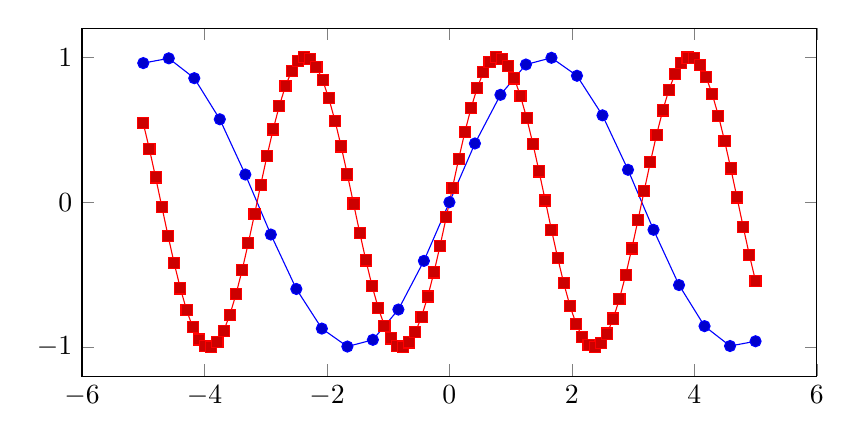
\begin{tikzpicture}
				\begin{axis}[
					width=0.9\textwidth,
					height=6cm,
					]
					
					\addplot {sin(deg(x))};
					\addplot+[samples=100] {sin(deg(2*x))};
				
				\end{axis}
			\end{tikzpicture}
			\caption{A nice sinus plot with Tikz.}
		\end{figure}
	\end{frame}
	
	% FRAME
	\begin{frame}{Bar charts}
		\begin{figure}
			\centering
			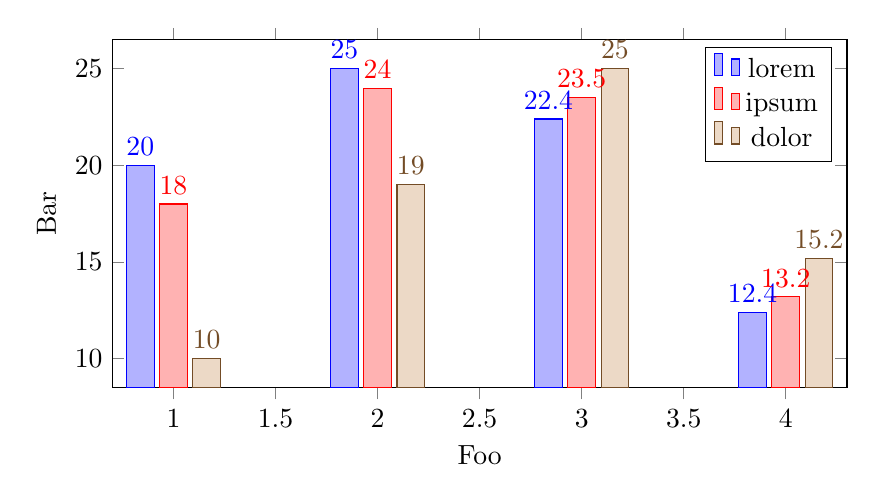
\begin{tikzpicture}
				\begin{axis}[
						ybar,
						xlabel={Foo},
					  	ylabel={Bar},
					  	width=0.9\textwidth,
					  	height=6cm,
						nodes near coords,
						nodes near coords align={vertical},
					]
					
					\addplot plot coordinates {(1, 20) (2, 25) (3, 22.4) (4, 12.4)};
					\addplot plot coordinates {(1, 18) (2, 24) (3, 23.5) (4, 13.2)};
					\addplot plot coordinates {(1, 10) (2, 19) (3, 25) (4, 15.2)};
					
					\legend{lorem, ipsum, dolor}
				
				\end{axis}
			\end{tikzpicture}
			\caption{A nice bar chart with Tikz.}
		\end{figure}
	\end{frame}
	
	% FRAME
	\begin{frame}{Quotes}
		\begin{quote}
			Veni, Vidi, Vici
		\end{quote}
		from Julius Caesar.
	\end{frame}
		
	% FRAME
	\begin{frame}[fragile]{References}
		Some references to showcase \verb|[allowframebreaks]| on next slide~\cite{Knuth92,ConcreteMath,Simpson,Er01,greenwade93}
	\end{frame}

	% % FRAME
	% \begin{frame}{References}
	% 	\bibliography{pres}
	% 	\bibliographystyle{abbrv}
	% \end{frame}

	% FRAME
	\begin{frame}[allowframebreaks]{References}
      \begin{thebibliography}{1}

         \bibitem{Er01}
         P.~Erd{\H o}s.
         \newblock A selection of problems and results in combinatorics.
         \newblock In {\em Recent trends in combinatorics (Matrahaza, 1995)}, pages 1--6. Cambridge Univ. Press, Cambridge, 1995.
         
         \bibitem{ConcreteMath}
         R.~Graham, D.~Knuth, and O.~Patashnik.
         \newblock {\em Concrete mathematics}.
         \newblock Addison-Wesley, Reading, MA, 1989.
         
         \bibitem{greenwade93}
         G.~D. Greenwade.
         \newblock The {C}omprehensive {T}ex {A}rchive {N}etwork ({CTAN}).
         \newblock {\em TUGBoat}, 14(3):342--351, 1993.
         
         \bibitem{Knuth92}
         D.~Knuth.
         \newblock Two notes on notation.
         \newblock {\em Amer. Math. Monthly}, 99:403--422, 1992.
         
         \bibitem{Simpson}
         H.~Simpson.
         \newblock Proof of the {R}iemann {H}ypothesis.
         \newblock preprint (2003), available at \texttt{http://www.math.drofnats.edu/riemann.ps}, 2003.
         
      \end{thebibliography}
   \end{frame}
	
\end{document}


\documentclass[aspectratio=169]{beamer}
\usetheme{gotham}

	\usepackage{standalone}
	\usepackage{tikz}
	\usepackage{pgfplots}
	\usepackage{tabularray} % Typeset tabulars and arrays (contains equivalent of longtable, booktabs and dcolumn at least) 
		\UseTblrLibrary{booktabs} % to load extra commands from booktabs
	\usepackage{changepage}

	\newcommand{\themename}{\textbf{\textsc{Gotham}}}


\begin{document} 

\section{Gotham Theme}

	% FRAME
	\begin{frame}[fragile]{Gotham}
	
		The \themename{} theme is a Beamer theme with a minimal-ish visual style largely inspired by the \href{https://github.com/matze/mtheme}{\textsc{Metropolis} Beamer Theme} by Matthias Vogelgesang (and some other Beamer themes).

		Yet, \themename{} is highly extendable and versatile.
		\bigskip
		
		First, enable the theme by classically loading it:
		
		\begin{verbatim}
			\documentclass{beamer}
			\usetheme{gotham}
		\end{verbatim}
		
		Then, the all customization can be performed at any moment in the presentation using:

		\begin{verbatim}
			\gothamset{<option>=...}
		\end{verbatim}
	\end{frame}


\subsection{Fonts}

	% FRAME	
	\begin{frame}[fragile]{Gotham title formats}
		Note, that you have to have Mozilla's \emph{Fira Sans} font and XeTeX or LuaTeX installed to enjoy this wonderful typography.

		\begin{columns}[T,onlytextwidth]
		\column{0.49\textwidth}
			\themename{} supports 4 different title formats \verb|\gothamset{format frametitle=}|
			\begin{itemize}
				\item regular
				\item \MakeLowercase{Lower}
				\item \MakeUppercase{Upper}
				\item \MakeTitlecase{Title Case}
			\end{itemize}
		\column{0.49\textwidth}
			\themename{} supports 3 different title shape \verb|\gothamset{shape frametitle=...}|:
			\begin{itemize}
				\item regular
				\item \textsc{Small caps}
				\item \textit{italic}
			\end{itemize}
		\end{columns}
		
		\vspace{2em}
		They can either be set at once for every title type or individually.
	\end{frame}

	{ \gothamset{shape frametitle=smallcaps, format frametitle=titlecase}
	% FRAME
	\begin{frame}{Titles: Small caps and titlecase}
		This frame uses the title format options: \texttt{shape frametitle=smallcaps, format frametitle=titlecase}.

		\begin{alertblock}{Potential Problems}
			Be aware that not every font supports small caps. 
			If for example you typeset your presentation with pdfTeX and the Computer Modern Sans Serif font, every text in small caps will be typeset with the Computer Modern Serif font instead.
			Please refer to the documentation if you consider using it.

			As a rule of thumb: just use it for plaintext-only titles.
		\end{alertblock}
	\end{frame}
	}

	{ \gothamset{format frametitle=upper, shape frametitle=italic}
	% FRAME
	\begin{frame}{Titles: Upper and italic}
		This frame uses the title format options: \texttt{format frametitle=upper, shape frametitle=smallcaps}.

		\begin{alertblock}{Potential problems}
			As this title format also uses small caps you face the same problems as with the \texttt{smallcaps} title format. 
			Additionally this format can cause some other problems. 
			Please refer to the documentation if you consider using it.
		\end{alertblock}
	\end{frame}
	}

	{ \gothamset{format frametitle=lower}
	% FRAME
	\begin{frame}{Titles: LOWER and regular}
		This frame uses the title format options: \texttt{format frametitle=lower, shape frametitle=regular}.
	\end{frame}
	}


\subsection{Colors}

	{ \gothamset{background=dark}
	% FRAME
	\begin{frame}[fragile]{Presentation style via background color}
		The color mode (a.k.a. background color) can be changed using:
		\begin{verbatim} \gothamset{background=dark | light | transparent} \end{verbatim}
	\end{frame}
	}

	% FRAME	
	\begin{frame}[fragile]{Blocks}
		Three different block environments are pre-defined and may be styled with an optional background color.
		
		\begin{columns}[T,onlytextwidth]
		 \column{0.3\textwidth}
		 	\begin{verbatim}\gothamset{
				block=native}\end{verbatim}

		   \begin{block}{Default}
		     Block content.
		   \end{block}
		
		   \begin{alertblock}{Alert}
		     Block content.
		   \end{alertblock}
		
		   \begin{exampleblock}{Example}
		     Block content.
		   \end{exampleblock}
		
		 \column{0.3\textwidth}
		
		   \gothamset{block=transparent}
			\begin{verbatim}\gothamset{
				block=transparent}\end{verbatim}
		
		   \begin{block}{Default}
		     Block content.
		   \end{block}
		
		   \begin{alertblock}{Alert}
		     Block content.
		   \end{alertblock}
		
		   \begin{exampleblock}{Example}
		     Block content.
		   \end{exampleblock}

		\column{0.3\textwidth}
		
		   \gothamset{block=fill}
			\begin{verbatim}\gothamset{
				block=fill}\end{verbatim}
		
		   \begin{block}{Default}
		     Block content.
		   \end{block}
		
		   \begin{alertblock}{Alert}
		     Block content.
		   \end{alertblock}
		
		   \begin{exampleblock}{Example}
		     Block content.
		   \end{exampleblock}
		
		\end{columns}
	\end{frame}

	% FRAME
	\begin{frame}[fragile]{Color customization}
		The colors can be changed using:
		\begin{verbatim}
		\colorlet{colorPale}{gPaleYell} % BG in light/normal mode
		\colorlet{colorDark}{gDarkBlack} % FG in light/normal mode
		\colorlet{colorA}{gDarkTeal} % frametitle, standin.out,
		\colorlet{colorAreversed}{gLightTeal} % frametitle, standin.in,
		\colorlet{colorB}{gMidGrey} % gray BG : progress bar, blocks
		\colorlet{colorC}{gDeepYellOr} % progress bar
		\colorlet{colorD}{gLightOrange} % alert
		\colorlet{colorE}{gLightGreen} % example 
		\end{verbatim}
	\end{frame}


\subsection{Inner}

	% FRAME
	\begin{frame}[fragile]{Title page}
		\themename{} offers the possibility to adapt the title page layout (printed with \verb|\maketitle| or \verb|\titlepage|).
		This can be achieved using:

		\begin{verbatim}   \defbeamertemplate{title page}{your name}{your defintion}
			\gothamset{title page= your name}\end{verbatim}
		
		\themename{} also predefined several templates such as: 
		\verb$gotham normal | gotham splitvert | gotham dividedpic$ \verb$| gotham reversed$
	\end{frame}

	% FRAME
	\begin{frame}[fragile]{Table of contents}
		\themename{} come with the possibility to apply different style for your table of contents (ToC) page.
		You can define your own ToC style as it follows:
		\begin{verbatim}
			\defbeamertemplate{toc page}{your name}{your def}
			\gothamset{tocframe template= your name}
		\end{verbatim}
		Then, referring to this template using the frame option \verb|[toc]| in your presentation: 
		\begin{verbatim}
			\begin{frame}[toc]{Table of contents}
				\tableofcontents%[hideallsubsections]
			\end{frame }\end{verbatim}

		Or using one of the \themename{} predefined template, such as: \verb$gotham simple | gotham bullet$
	\end{frame}

	% FRAME
	\begin{frame}[fragile]{Sections}
		\themename{} provides a multiple options to tune sections (respectively \verb|part|, \verb|section|, \verb|subsection| and \verb|subsubsection|).
		Thus, using the setting controls:
		
		The section command \verb|\section{Elements}| from Beamer will appear very differently.
		The section page will appear or disappear thanks to: \verb$\gothamset{sectionframe default=<on|off>}$, while its layout (when appearing) is controlled by: 
		\begin{verbatim}
			\defbeamertemplate{part|sub|subsub|section frame}
				{your name}{your def}
			\gothamset{sectionframe template= your name}\end{verbatim}

		\themename{} predefined template are: \verb$gotham progressbar | gotham simple |$ \verb$gotham splitvert progressbar |$ \verb$gotham splitvert simple | gotham progressvert$
	\end{frame}

	% FRAME
	\begin{frame}[fragile]{Sections contents}
		After the section page, you can (de)activate a page with table of contents in the section using \verb$\gothamset{sectiontocframe default=<on|off>}$, and its layout is controlled by: 
		\begin{verbatim}
			\defbeamertemplate{toc subsection frame}{your name}{your def}
			\gothamset{sectionframe template= your name}
		\end{verbatim}

		\themename{} predefined template are: \verb$gotham simple | gotham bullet$
	\end{frame}

	% FRAME
	\begin{frame}[fragile, watermark]{Watermark}

		With \themename{} you can locally or globally add watermark to your slides by using:
		\begin{verbatim}  \defbeamertemplate{background}{watermark/your name}{your def}
		  \gothamset{watermark template= your name}\end{verbatim}
		
		Then, this watermark can be turn on locally using \verb|\begin{frame}[watermark]| or globally with \verb|\gothamset{watermark default= on}| .
 	\end{frame}

	% FRAME
	\begin{standinenv}
	\begin{frame}[fragile]{Standin}

		\themename{} comes with 2 environments/specials layouts named \verb|standin| and \verb|standout|.
		These specials layouts can be used to emphasize some content or last slide\textellipsis

		This layout can be turn on using \verb|\begin{frame}[standin]| or using the dedicated environment (\verb|\begin{standinenv}\begin{frame}...\end{frame}\end{standinenv}|).

		Note that the background can also be tuned using:
		\begin{verbatim}  \defbeamertemplate{background canvas}{standin/name}{your def}
		  \gothamset{standin template= name}\end{verbatim}
		
	\end{frame}
	\end{standinenv}

	% FRAME
	\begin{frame}[standout, watermark]{Standout}
		Here is an example of standout (working as standin), that can be combined with a watermark.

		Another difference, apart the obvious color change is the font size and series.
	\end{frame}


\subsection{Outer}
	
	{%
		\setbeamertemplate{frame footer}{My custom footer}
	% FRAME
	\begin{frame}[fragile]{Frame footer}
	   \themename{} defines a custom Beamer template to add a text to the footer. 
		It can be set via
	   \begin{verbatim}\setbeamertemplate{frame footer}{My custom footer}\end{verbatim}

		Even after redefining (or not) your frame footer template, you can locally remove it with the frame option \verb|\begin{frame}[nofooter]|.
	\end{frame}
	}

	\title[your shorttitle]{Gotham}
	\date[shortdate]{\today}
	\author[your shortauthor name]{Romain NOËL}
	% FRAME
	\begin{frame}[fragile, rotateFooter]{rotateFooter}
		The default footer from \themename{}, it displays the \verb|shortdate|, \verb|shorttitle| and \verb|shortauthor|.
		So by filling these fields in your document setup, you will see them appear in your footer:
		\begin{verbatim}   \title[your shorttitle]{Your title}
			\date[shortdate]{\today}
			\author[your shortauthor name]{John DOE} \end{verbatim}

		Since, we always need some extra space on some frames that would like to overlay a bit the footer, \themename{}'s footer offers also possibility to be put on side locally using \verb|\begin{frame}[rotateFooter]|, or globally with 
		\begin{verbatim} \gothamset{rotateFooter default=on} \end{verbatim}
		If it has set globally, it can be deactivated locally with the frame option \verb|\begin{frame}[norotateFooter]|.
	\end{frame}

	\title[]{Gotham}
	\date[]{\today}
	\renewcommand{\gothamRightFiligrane}{%
		\rotatebox{90}{gotham right filigrane pattern}
	}
	% FRAME
	\begin{frame}[edging, fragile]{Edging}
		\themename{} has two hook commands, \verb|\gothamRightFiligrane| and \verb|\gothamLeftFiligrane|, that can be redefined to customize what to display in the edgings (a.k.a. filigrane, a.k.a. sidebar).
		As example, one could do:
		\begin{verbatim}
			\renewcommand{\gothamRightFiligrane}{%
				\rotatebox{90}{gotham right filigrane pattern}
			}\end{verbatim}

		Then, to set if it should be displayed or not, globally \begin{verbatim} \gothamset{edging default=on} \end{verbatim}
		or locally with the frame option \verb|\begin{frame}[edging]| or \verb|\begin{frame}[noedging]|.
	\end{frame}

	% FRAME
	% \begin{nofootlineenv}
	\begin{frame}[fragile,noedging,nofooter]{Really wide contents}
		\begin{adjustwidth}{-2em}{-2em}
			If you want a really wide content in your frame, you can change the size of your margin (requires \verb|\usepackage{changepage}| in your preamble).
			You can also suppress the edging (\verb|[noedging]|) and footer (\verb|[nofooter]|) or even more radically footline (\verb|[nofootline]|).

			Here is an example combining them: 
			\begin{verbatim}
				\begin{frame}[noedging,nofootline]{extended frame}
					\begin{adjustwidth}{-2em}{-2em}% 2em extra to the left and 2em for right margin.
						wide content
					\end{adjustwidth}
				\end{frame }
			\end{verbatim}
		\end{adjustwidth}
	\end{frame}
	% \end{nofootlineenv}

	{%
	\renewcommand{\gothamInstituteLogoSquare}[1][4ex]{%
      
\includegraphics[height=#1]{gotham-logo.pdf}
   }
	\logo{extra LOGO}
	% FRAME
	\begin{frame}[fragile]{Frametitle}
		\framesubtitle{with a subtitle}
		The frametile template brought by \themename{} is relatively classic: it supports \verb|\subframetitle| and frame continuation (with \verb|[allowframebreaks]|) through templates that can be tuned.
		Nevertheless, it the frametitle template also includes a hook for your institute logo in the top right corner, leaving the command \verb|\logo{}| free for your extra logos.
		
		So, one can have both logos using:
		\begin{verbatim}
			\renewcommand{\gothamInstituteLogoSquare}[1][4ex]{
				
\includegraphics[height=#1]{gotham-logo.pdf}
			}
			\logo{extra LOGO}
		\end{verbatim}
	\end{frame}
	}

	\author[]{Romain NOËL}
	{%
		\gothamset{progressbar position=foot, numbering= totalframenumber}
	% FRAME
	\begin{frame}[fragile]{Numbering and progressbar}

		\themename{} theme can numbering your frames in the bottom right corner using different styles. 
		You can also decide to use a progression bar to indicate how much of your presentation remains.

		The setup of numbering and progression bar can be performed through:
		\begin{verbatim}
			\gothamset{numbering= totalframenumber, progressbar position=foot}
		\end{verbatim}

		Numbering available options are: \verb$none | framenumber | totalframenumber | appendixframenumber | pagenumber | totalpagenumber | circle$

		Progressbar position available options are: \verb$none | head | frametitle | foot | circlehead$
	\end{frame}
	}


\end{document}
%EoF

\documentclass[aspectratio=169]{beamer}
% \usetheme{gotham}

   \usepackage{appendixnumberbeamer}
   \usepackage[scale=2]{ccicons}
   \newcommand{\themename}{\textbf{\textsc{Gotham}}}


\begin{document}

\section{Conclusion}

	% FRAME
	\begin{frame}{Summary}
		Get the source of this theme and the demo presentation from

		\begin{center}\url{https://gitlab.com/RomainNOEL/beamertheme-gotham}\end{center}

		The theme \emph{itself} is licensed under a \href{http://creativecommons.org/licenses/by-sa/4.0/}{Creative Commons Attribution-ShareAlike 4.0 International License}.
		\begin{center} \ccbysa \end{center}
	\end{frame}

	% FRAME
   \begin{standoutenv}
   \begin{frame}[fragile]
      The final slide using the standout style with command:
		\begin{verbatim}
			\begin{frame}[standout, plain]{Thank You !}
				Questions ?
		 	\end{frame }
		\end{verbatim}

		\begin{center}
			Et voilà !
		\end{center}
   \end{frame}
   \end{standoutenv}
	
\end{document}



%%%%%%%%%%%%%%%%%%%%
%%%  BACKMATTER  %%%
%%%%%%%%%%%%%%%%%%%%

	% FRAME
	\begin{frame}[noframenumbering, allowframebreaks]{References}
		\printbibliography[heading=none]
		% \bibliography{demo}
		% \bibliographystyle{abbrv}
	\end{frame}


%%  APPENDIX  %%
%%%%%%%%%%%%%%%%
\appendix
% \miniframesoff % to deactive the navigation bar requires ()

	% FRAME
	\begin{frame}[fragile]{Backup slides}
		Sometimes, it is useful to add slides at the end of your presentation to refer to during audience questions.

		The best way to do this is to include \verb|\usepackage{appendixnumberbeamer}| in your preamble and call \verb|\appendix| before your backup slides.
	\end{frame}

\sectionpic{BeamerExtra}{\PathSO/Logos/UGE-logo.pdf}
	
	\begin{frame}[fragile]{Backup slides}
		Sometimes, it is useful to add slides at the end of your presentation to
		refer to during audience questions.
		
		The best way to do this is to include the \verb|appendixnumberbeamer|
		package in your preamble and call \verb|\appendix| before your backup slides.
		
		\themename will automatically turn off slide numbering and progress bars for
		slides in the appendix.
	\end{frame}
	
	\begin{frame}[fragile, label=previouSlide]{Section With Pictures}
		As the following command indicates, it is possible to include pictures under a section title:
		\begin{verbatim}			
			\sectionpic{BeamerExtra}{\PathSO/Logos/UGE.pdf}		
		\end{verbatim}
	\end{frame}

	\begin{frame}[fragile]{Section Content}
		The table of content after the section slide can be turn on or off with the command:
		\begin{verbatim}
			\boolfalse{sectionContent} % to turn off the table of content.
		\end{verbatim}
	
		From example, the table of content will be turn of for the next section (on the following slide).

		The name the content slide can also be modified thanks to the command:
		\begin{verbatim}
			\renewcommand{\secContentName}{def} % to redefine the title on section content.
		\end{verbatim}
	\end{frame}
	
	\renewcommand{\secContentName}{refined name}
	\boolfalse{sectionContent}
\section{Things good to know about Beamer (not BeamerExtra)}
	\booltrue{sectionContent}
	
	\begin{frame}[fragile]
		\frametitle{link to hidden slide}
		
		Thanks to Beamer, you can create buttons to just to hidden slides that are in the appendices
		\begin{verbatim}			
			\begin{frame}[label=<originalSlide>, noframenumbering]	
			\hyperlink{<hiddenSlide>}{\beamerbutton{NameOfButton}}
		\end{verbatim}
		
		Don't forget to create a button to come back also!
		
		For example :
		\hyperlink{previouSlide}{\beamerbutton{back to previous slide !}}
	\end{frame}
	
	\begin{frame}<all:1>[fragile]
		\frametitle{Print extended version}
		\framesubtitle{1}
		
		This slide will always be printed with 
		\begin{verbatim}			
			\begin{frame}<handout:1|beamer:1> or \begin{frame}<all:1>
		\end{verbatim}
		
		while the following code will never appears
		\begin{verbatim}			
			\begin{frame}<handout:0|beamer:0> or \begin{frame}<all:0>	
		\end{verbatim}
	\end{frame}
	
	\begin{frame}<handout:0|beamer:1>[fragile]
		\frametitle{Print extended version}
		\framesubtitle{2}
		
		This frame will appear with
		\begin{verbatim}			
			\documentclass[]{beamer}
			\begin{frame}<handout:0|beamer:1>
		\end{verbatim}
		
		BUT the following will not appear
		\begin{verbatim}			
				% requires handout to appear
				\documentclass[10pt]{beamer} 
				\begin{frame}<handout:1|beamer:0>
		\end{verbatim}
		
		BY opposition with \begin{verbatim} \documentclass[handout]{beamer}
		\end{verbatim}
	\end{frame}
			
	\begin{frame}<handout:1|beamer:0>[fragile]
		\frametitle{Print extended version}
		\framesubtitle{2}
		
		This frame will appear with
		\begin{verbatim}			
			\documentclass[handout]{beamer}
			\begin{frame}<handout:1|beamer:0>
		\end{verbatim}
		
		BUT the following will not appear
		\begin{verbatim}			
		    % requires to remove handout to appear
			\documentclass[handout]{beamer} 
			\begin{frame}<handout:0|beamer:1>
		\end{verbatim}
		
		BY opposition with \begin{verbatim} \documentclass[]{beamer}
		\end{verbatim}
	\end{frame}
	

\section{Things brought by good practices in UserPackage}

	\begin{frame}
		\frametitle{nTheorem}

		The interactions beteween ntheorem and beamer has been solved.

		\begin{theorem}
			contenu...
		\end{theorem}

		\begin{proof}
			contenu...
		\end{proof}
	\end{frame}

	\begin{frame}
		\frametitle{Glossaries}

		Here is an example of acronym using glossaries: \gls{lbm}

		And an example of equation in colors, the Boltzmann equation:
		\begin{equation}
			{\color{blue} \partial_t \gls{BoltzDist}(x,\xi,t)} + {\color{red} \xi\cdot\partial_x \gls{BoltzDist}(x,\xi,t)} + {\color{green!60!black!80} g\cdot\partial_\xi f(x,\xi,t)}
			= {\color{yellow!80!orange!85!black} \Omega(\gls{BoltzDist},\gls{BoltzDist})}
		\end{equation}
		where $\gls{BoltzDist}$ is a variable defined through glossaries.

	\end{frame}

	\begin{frame}[fragile]
		\frametitle{Cite in the footnote}

		Some text that requires a reference\footfullciteBeamer{Knuth92},
		using the command\footnote{Please note that this command can be used side-by-side the command footnote.}
		\begin{verbatim}
				\footfullciteBeamer{<bibKey>}
		\end{verbatim}

		The command to cite in text mode is also possible with
		\begin{verbatim}
				\fullciteBeamer{<bibKey>}
		\end{verbatim}
		and giving \fullciteBeamer{ConcreteMath}
	\end{frame}

	\begin{frame}%[fragile]
		\frametitle{Video using media9/multimedia}

		\begin{columns}[c,onlytextwidth]
		\column{0.49\textwidth}
		
			The last but not least feature present is a macro simplifying the way to include videos in beamer presentation.

			It requires to define the OS on which the pdf will be red, thanks to the command:
			\begin{center}
				\ttfamily
				\textbackslash def\textbackslash OSvar\{linux\}
			\end{center}

			Then, the video can be included with the command:\\[0.25em]
			\begin{flushleft}
				\ttfamily
				\textbackslash includeVideo[\% no space\\
				\qquad width=7cm, height=5cm,%\\
				]\% Options \\
				\{\textbackslash PathS/video.mp4\}\% Video File\\
				\{\textbackslash includegraphics[width, height]\%\\
				\qquad	\{\textbackslash PathS/screenshot.png\}\%\\
				\}\% Poster image.
			\end{flushleft}

		\column{0.49\textwidth}
			Leading to the following result:

			\begin{figure}
				\centering
				\includeVideo[% no space
						width=0.75\linewidth, height=0.54\linewidth,
					]% Options
					{\PathS/Air_convec.mp4}% Video File
					{\includegraphics[width=0.75\linewidth,height=0.54\linewidth]%
						{\PathS/Thermal_convec.png}%
					}
				\caption{Example of embedded video using \texttt{\textbackslash includeVideo}.}
				\label{vid:includeVideo}
			\end{figure}
		\end{columns}
	\end{frame}

	\begin{frame}[fragile]{Warning about \texttt{\textbackslash includeVideo}.}
		\begin{alertblock}{Warning}
			Currently the method to include video using \texttt{\textbackslash includeVideo} is no longer work on Windows because \texttt{flash player} is no longer supported.
		\end{alertblock}
		Up to now, this solution is still working on Linux with \texttt{okular}, \texttt{poppler} and \texttt{phonon-backend-vlc} installed.

		A possible workaround is to used external player rather than embedded solutions.
		An example of external inclusion on Windows with \texttt{multimedia} package is:
		\begin{verbatim}
			\movie[externalviewer]%
	   {\includegraphics[width=\textheight]%
	      {figures/image.jpg}%
	   }{video_beamer.mp4}
		\end{verbatim}
	\end{frame}


	\newcounter{r}
	\newcommand{\escalar}[1]{
	\setcounter{r}{#1 * #1 * #1}
	}
	%
	\newcounter{m}
	\setcounter{m}{0}
	\newcounter{mc}
	%
	\begin{frame}[fragile]{Video using animate}

		\vspace{-2em}
		\begin{columns}[c,onlytextwidth]
		\column{0.49\textwidth}

			Another solution which is use a animation from a stack of image:
			\begin{verbatim}
				\animategraphics[autoplay, loop,
				   	width=\textwidth, controls
					]%
				{<frame rate>}}{Images/Image_}{0}{99}
			\end{verbatim}
			or for more complex drawing:
			\begin{verbatim}
				\begin{animateinline}[<opt>]{<rate>}
		   ... typeset material ...
				\newframe[<frame rate>]
		   ... typeset material ...
				\newframe
		   ...
				\end{animateinline}
			\end{verbatim}
		\column{0.49\textwidth}
			\begin{figure}
				\centering
				\begin{animateinline}[loop, poster = first, controls, palindrome]{2}
					\whiledo{\them < 21}{
		    \begin{tikzpicture}[scale=0.95]
			   \draw[red,thick,<->] (-1,1) parabola bend (0,0) (2.1,4.41)
			       node[below right] {$y=x^2$};
			   \draw[loosely dotted] (-1,0) grid (4,4);
			   %\path[use as bounding box] (-2,-1) rectangle (5,5);
			   \draw[->] (-0.2,0) -- (4.25,0) node[right] {$x$};
			   \draw[->] (0,-0.25) -- (0,4.25) node[above] {$y$};
			   \foreach \x/\xtext in {1/1, 2/2, 3/3}
			   \draw[shift={(\x,0)}] (0pt,2pt) -- (0pt,-2pt) node[below] {$\xtext$};
			   \foreach \y/\ytext in {1/1, 2/2, 3/3, 4/4}
			   \draw[shift={(0,\y)}] (2pt,0pt) -- (-2pt,0pt) node[left] {$\ytext$};
						%
			   \setcounter{mc}{\value{m}*\value{m}}
			   \shade[top color=blue,bottom color=gray!50]
			       (0,0) parabola (0.1*\them,0.01*\themc) |- (0,0);
			   \escalar{\them}
			   \draw (3cm,2pt) node[above]
			       {$\displaystyle\int\limits_0^{\them/10} \!\!x^2\mathrm{d}x =
			           \displaystyle\frac{\ther}{3000}$};
			   \draw[fill=orange,color=orange] (0.1*\them,0.01*\themc) circle (0.5pt);
		   \end{tikzpicture}
				%
				\stepcounter{m}
				\ifthenelse{\them < 21}{
					\newframe
				}{
				\end{animateinline}\relax % BREAK
				} } % END \whiledo...
				\caption{Example of embedded video using \texttt{\textbackslash animategraphics}.}
				\label{vid:animate}
      	\end{figure}
     	\end{columns}
	\end{frame}



\addtocounter{levelstanda}{-1}
\end{document}
% EoF